\documentclass{article}
\usepackage{graphicx} % Required for inserting images
\usepackage{amsmath}
\usepackage{placeins}
\usepackage{listings}
\title{Final Project 456}
\author{Willem Strydom }
\date{December 14 2023}

\renewcommand{\thesection}{\arabic{section}}
\setcounter{section}{-1}
\begin{document}

\maketitle

\section{Introduction}
This project analyzes Verizon Communications Inc.'s common stock (NYSE: VZ).

Stock spot price and call price premiums data necessary for the analysis were collected from Yahoo Finance, and macroeconomic indicators (R) were collected from the U.S. Treasury Department website on the evening of Sunday, Dec $10^{th}$.

\section{Implied Volatility}
The IV displayed on yahoo finance for various calls is as follows. The data is for trading which stopped on 12/8. Time to expiry is listed in weeks on the top, and the strike price, in dollars, is on the rows
\FloatBarrier
$$
\begin{bmatrix}
strike/expiry& 1 & 2 &  & 3 & 4\\
39&0.1875 & 0.1753 & 0.1699 & 0.1729 & 0.1631\\
40&0.2266 & 0.1895 & 0.1690 & 0.1699 & 0.1548\\
41&0.2656 & 0.2168 & 0.1856 & 0.1816 & 0.1719\\
42&0.4492 & 0.4482 & 0.2070 & 0.2402 & 0.1953\\
43&0.4063 & 0.2813 & 0.2500 & 0.4575 & 0.3643\\
\end{bmatrix}
$$
\begin{figure}
    \centering
    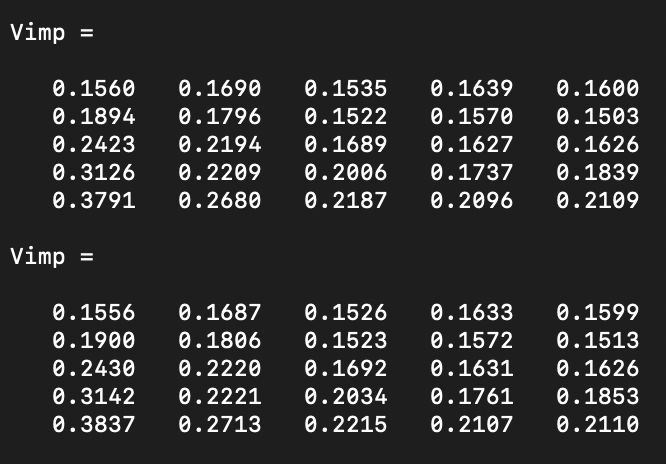
\includegraphics[width=0.8\linewidth]{crrvsbs.png}
    \caption{Comparison of IV calc by BS (top) vs CRR(bottom)(depth = 40)}
    \label{IV comparison of bs (top) vs crr(bottom)}
\end{figure}
\FloatBarrier
The implied volatility calculated by using BS() and CRRa() from the class website in \ref{app:appendix1} is not different by more than $1\%$ for any strike/expiry combination sampled. The observed difference is due to the depth of the binomial tree used in the CRR model. By increasing the depth of the tree, we will reduce the difference in implied volatility.\\
\hspace*{0.5cm}The implied volatility that is priced is always higher than what we calculate using both CRR and BS models. This is because the seller of an option wishes to make money, so the price reflects a higher volatility than can be reasonably observed.
\FloatBarrier
\begin{figure}
    \centering
    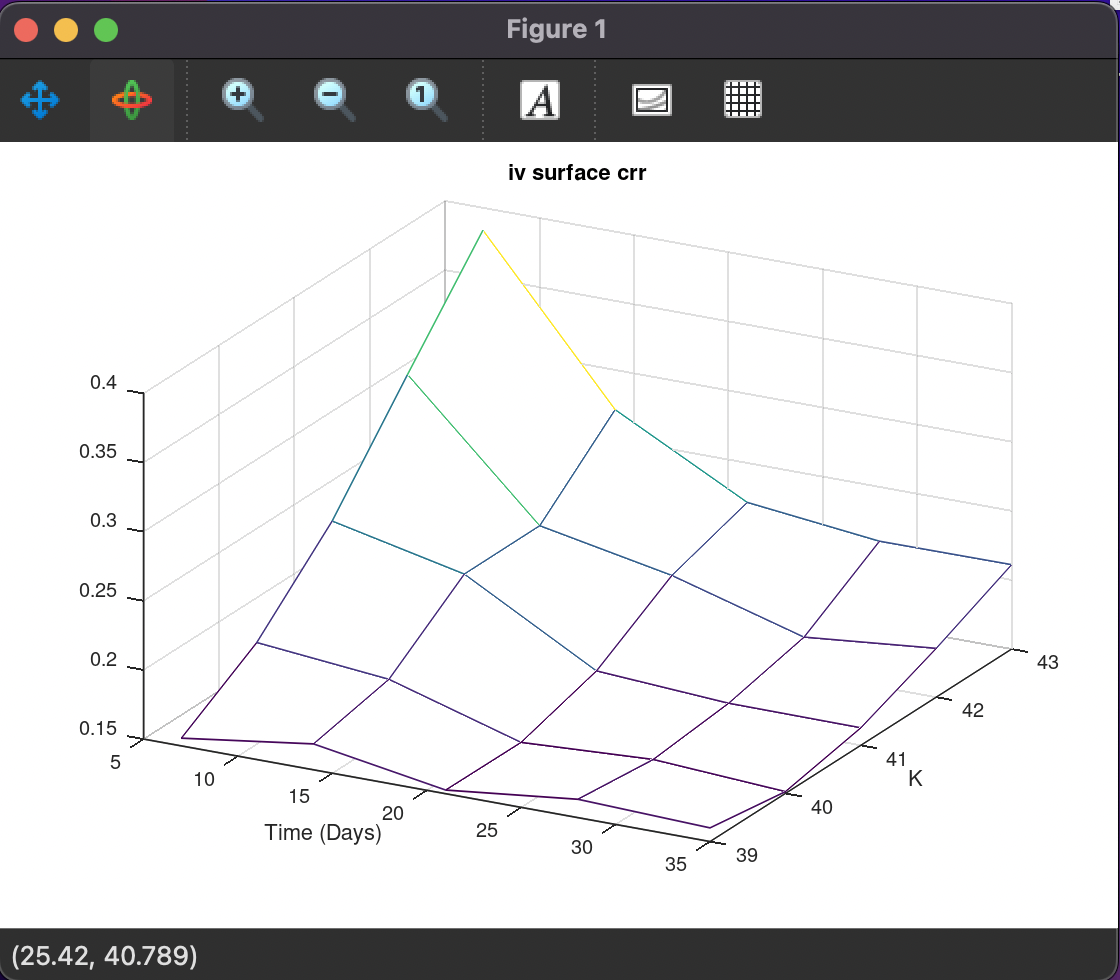
\includegraphics[width=0.8\linewidth]{crr.png}
    \caption{Comparison of IV calc by BS (top) vs CRR(bottom)(depth = 40)}
    \label{IV comparison of bs (top) vs crr(bottom)}
\end{figure}
\FloatBarrier
\begin{figure}
    \centering
    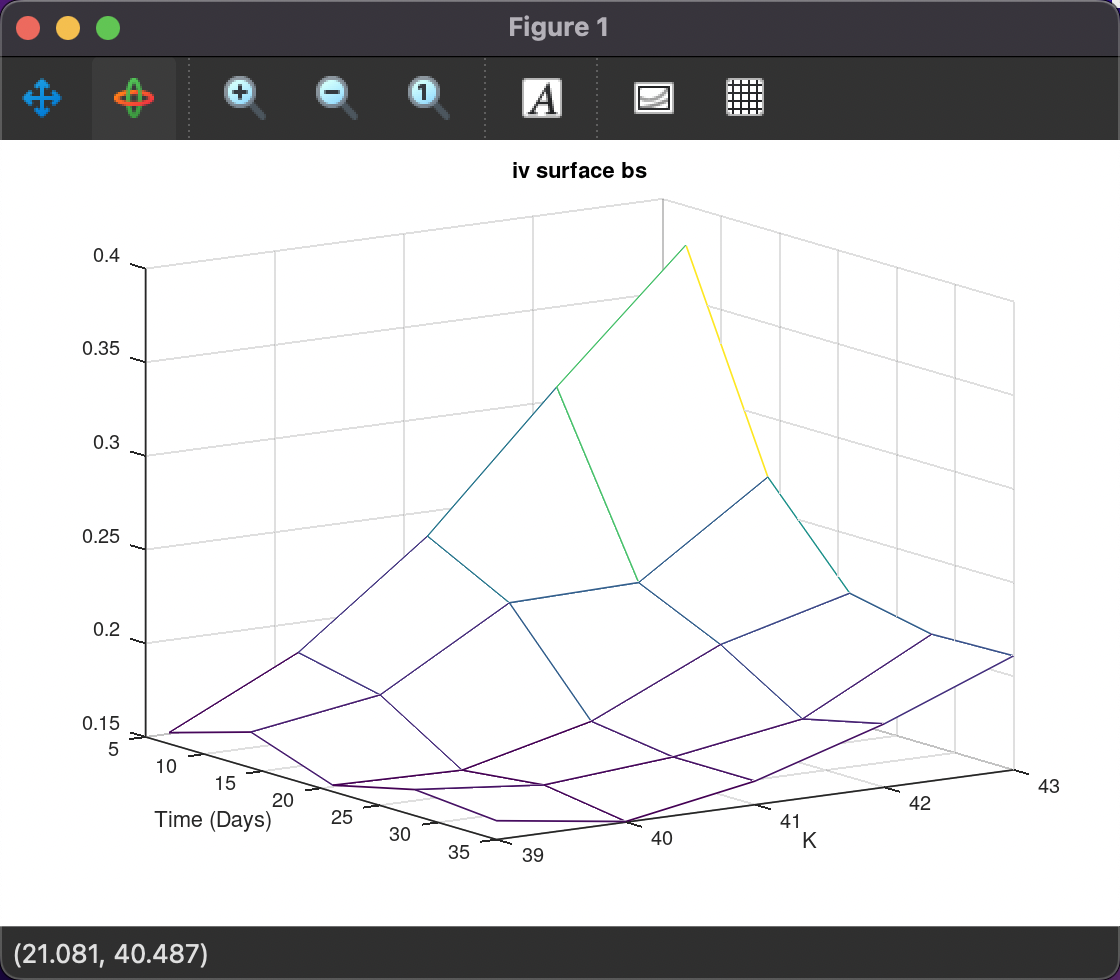
\includegraphics[width=0.8\linewidth]{bs.png}
    \caption{Comparison of IV calc by BS (top) vs CRR(bottom)(depth = 40)}
    \label{IV comparison of bs (top) vs crr(bottom)}
\end{figure}
\FloatBarrier
\section{Derivatives of Dividend Paying Stocks}
\hspace*{0.5cm}Let T = 1.1 year, K = 40, S0 = 38.28., r = 0.0527 There are typically 4 quarterly dividends of 0.66 cents payed out during this time period. We will calculate the implied volatility of a call option with the same strike and expiry 1 year, 1 month and 6 days from now to estimate the volatility $v$ that will be used in our model. We use the code in \ref{app:appendix2} along with CRRa(), CRRDaec(), and CRRDaep() to compute:
\\
\\
American Call Price (K = 40): 1.6119 (ours)\\
American Call Price (K = 40): 1.90 (listed last price)\\
American Put Price (K = 35):  1.2584 (ours)\\
American Put Price (K = 35):  1.3191 (listed last price)\\

The listed prices for call and put options with same strike and expiry expiry T = 1 year, 1 month and 6 days are both significantly higher that our calculated prices with the same strike and nearly same time to expiry.
\\
After changing the 2nd dividend to be 1.2 times the first, we calculate different call and put premiums as follows:
\\
American Call Price (K = 40): 1.5899\\
American Put Price (K = 35):  1.2937 \\
\hspace*{0.5cm}This shows that increasing the second dividend amount makes a call option less valuable, and a put more valuable. This is because the increased dividend amount make the early exercise of a call option desirable, as the holder of the call wishes to be given the dividend even more now, where as the opposite is true for a put option.

\section{Implied Binomial Tree W/O dividends}
\hspace*{0.5cm}We will use IBT123j() from the class website as in \ref{app:appendix3} to compute an implied binomial tree $"S"$, as well as tree $"Q"$ of probabilities for each state in the tree. The value of a put can then be calculate by calculating the expectation of the put payoff at expiry:

$$P(0,k) =E_j([k - S(T,j)]^+) = Max([k - S(T,j)]^+, 0) * Q(T,j)$$
\FloatBarrier
\begin{figure}
    \centering
    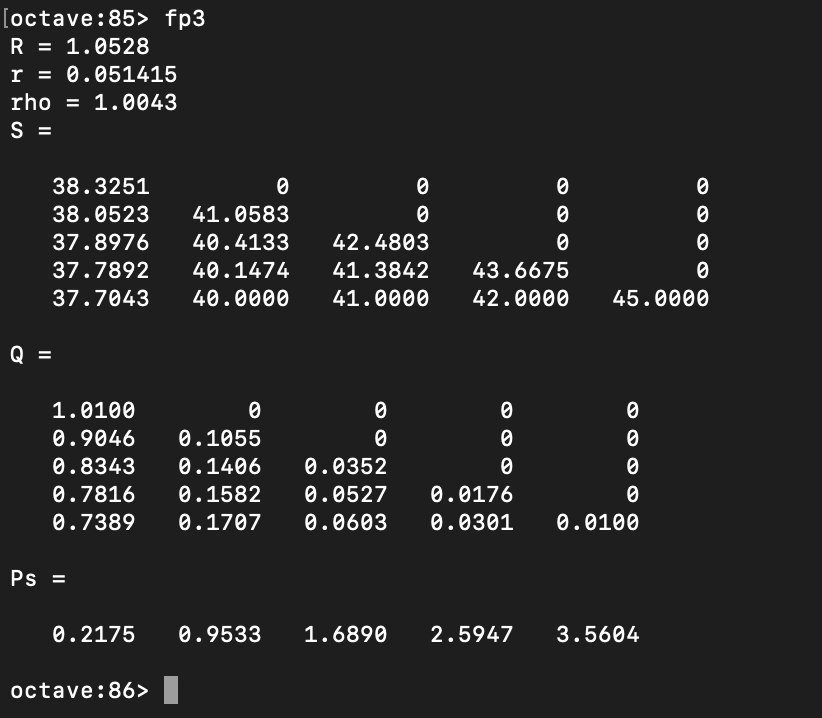
\includegraphics[width=0.8\linewidth]{part3out.png}
    \caption{output from (3)}
    \label{IV comparison of bs (top) vs crr(bottom)}
\end{figure}
\FloatBarrier
The listed Put last prices for the same strikes and expiry 1 month from the date of data collection are given as:
$$
\begin{bmatrix}
    k: & 38 & 39 & 40 & 41 & 42\\
    Price: & 0.44 & 0.88 & 1.76 & n/a & 3.73\\
    Ours: & 0.22 & 0.95 & 1.69 & 2.59 & 3.56
    
\end{bmatrix}
$$
Note: there was not a listing for a put with $k = 41$ for the chosen expiry date.\\
\\
\hspace*{0.5cm}These prices are mostly in accordance with what we have seen earlier in this project in that the option is being traded at a slightly higher price than we calculate using our models.
\\
\\
When comparing with values given by the call put parity formula:
$$
P = -S + \frac{k}{(1+r)^T} + C
$$
with $r = 0.0514$, as in our model, we find \\
$$
\begin{bmatrix}
    Source/k: & 38 & 39 & 40 & 41 & 42\\
    Market: & 0.44 & 0.88 & 1.76 & n/a & 3.73\\
    Ours: & 0.22 & 0.95 & 1.69 & 2.59 & 3.56\\
    CPP: & 0.48 & 0.96 & 1.69 & 2.60 & 3.56
\end{bmatrix}
$$
\hspace*{0.5cm}The call put parity prices are almost exactly the prices given by recombining binomial tree model $("Ours")$ except for k = 39. This is likely due to the fact that the binomial tree from IBT123j() does not include any states between 38 and 39, so the price for a put with k = 39 is going to be higher than it probably should be.
\newpage
\appendix
\section{Implied Volatility}
\label{app:appendix1}
\begin{lstlisting}
Ks = [39,40,41,42,43];
Ts = [7,14,21,28,35];
C = [0.09,.02,.01,.01,.01;
.23,.07,.04,.01,.01;
.28,.08,.03,.02,.01;
.4,.14,.05,.02,.02;
.46,.17,.08,.05,.04;
];
C = C'
Rs = [5.29,5.28,5.27,5.26,5.28]; %4week t-ball rates from 12/04-08/23
r = mean(Rs);

S0 = 38.28;r = 0.215;
Vimp = zeros(length(Ks),length(Ts));
minv = 0.01;maxv = 0.99;
tol = 0.00001;
for col = 1:length(Ts)
  T = Ts(col)/365;
  for row = 1:length(Ks)
    f = @(v) BS(T,S0,Ks(row),r/100,v);
    Vimp(row,col) = bisection(f,C(row,col),minv,maxv,tol);
  endfor
endfor
%display meshgrid and matrix
mesh(Ts,Ks,Vimp);
title('iv surface bs');
xlabel('Time (Days)');
ylabel('K');
Vimp
for col = 1:length(Ts)
  T = Ts(col)/365;
  for row = 1:length(Ks)
    g = @(v) CRRa(T,S0,Ks(row),r/100,v,40);
    Vimp(row,col) = bisection(g,C(row,col),minv,maxv,tol);
  endfor
endfor
%display meshgrid and matrix
mesh(Ts,Ks,Vimp);
title('iv surface crr');
xlabel('Time (Days)');
ylabel('K');
Vimp
\end{lstlisting}
\section{Dividends}
\label{app:appendix2}
\begin{lstlisting}
S0 = 38.28;r = 0.215; 
Di = 0.66*[0,0,1,0,0,1.2,0,
      0,1,0,0,1,0,0]; %quarterly dividends of 66 cents
T = 1.1;
K = 40;
Rs = [5.29,5.28,5.27,5.26,5.28]; %4week t-bill rates from 12/04-08/23
r = mean(Rs);
r = r/100;
N = 12;
minv = 0.01;maxv = 0.99;
tol = 0.00001;
g = @(v) CRRa(T,S0,K,r/100,v,N); %calculate volatility implied by listed options
v = bisection(g,1.9,minv,maxv,tol);
[Ca,Ce,EE]=CRRDaeC(T,S0,K,Di, r,v,N);
Ca(1,1)
K = 35;
[Pa,Ce,EE]=CRRDaeP(T,S0,K,Di, r,v,N);
Pa(1,1)

\end{lstlisting}
\section{Call-Put Parity}
\label{app:appendix3}
\begin{lstlisting}
S0=38.28; Ks=39:44; % VZ spot price and strikes

Cs=[40,14,5,2,2,1]/100; % Call last prices
Rs = [1.0529,1.0528,1.0527,1.0526,1.0528]; %APR from 4 week t bills
R = mean(Rs);
R
r = log(R);
r
rho = exp(r/12); % not super sure if calculating rho correctly: ~1 month to expiry
rho
w = @(x)x;
[S,Q,up,down,pu,N1] = IBT123J(S0,Ks,Cs,rho,w);
%computing put prices:
S
Q
%use Q to calculate expectd value of each put at expiry, without having to do 
% the backwards induction I think...
%Pk = [S0 - k]+
ST = S(end,:); # for init of W tree
Qs = Q(end,:);
i = 1;
Ps = zeros(1,5);
% use constant R because lazy
for k = 38:42 % can only find real puts with even dollar strikes for given expiry
  val = 0;
  for j = 1:5 % S vals at expiry
    val = val + max(k - ST(j),0) * Qs(j); % expected value of each put according to S and Q
    
  endfor
  val = val/rho; %adj for time val of money
  Ps(i) = val;
  i = i+1;
 endfor
Ps

%calc ps from CPP formula

CPPS = zeros(1,5)
Ks = 38:42
Cs = [.92,.4,.14,.05,.02] % call prices with matchin strikes and expiries
for i =1:5
  CPPS(i) = Cs(i) + Ks(i)/((1+r)^(1/12)) - S0;
endfor
CPPS
  


\end{lstlisting}
\end{document}
